%----------------------------------------------------------------------------------------
%	CHƯƠNG 4: KẾT QUẢ THỰC NGHIỆM VÀ NHẬN XÉT
%----------------------------------------------------------------------------------------

\chapter{KẾT QUẢ THỰC NGHIỆM VÀ NHẬN XÉT}
\label{Chapter4}

% =================================================================
%   MỤC 4.1
% =================================================================
\section{Kết quả thiết kế giao diện}
\begin{center}
	\nopagebreak
	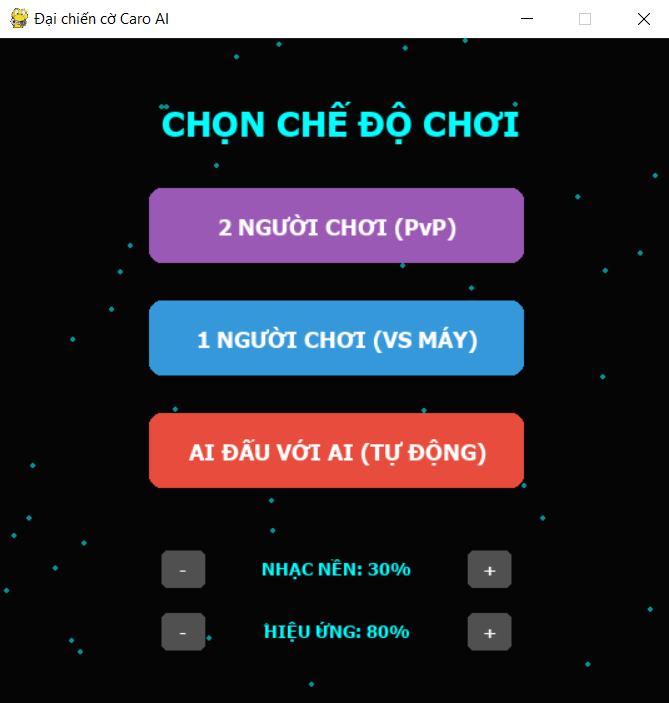
\includegraphics[width=\textwidth]{Figures/Gallery/mode.png}
	\captionof{figure}{Màn hình Menu cấu hình chế độ chơi}
	\label{fig:mode_choosin}
\end{center}
\vspace{0.3cm}
\textbf{Màn hình Chọn chế độ chơi:} Giao diện sử dụng hiệu ứng các hạt trôi nổi tạo chiều sâu không gian. Hệ thống cung cấp 3 chế độ chơi: 2 Người chơi (PvP), 1 Người chơi với máy (PvE), cho AI tự đấu (EvE).
\begin{center}
	\nopagebreak
	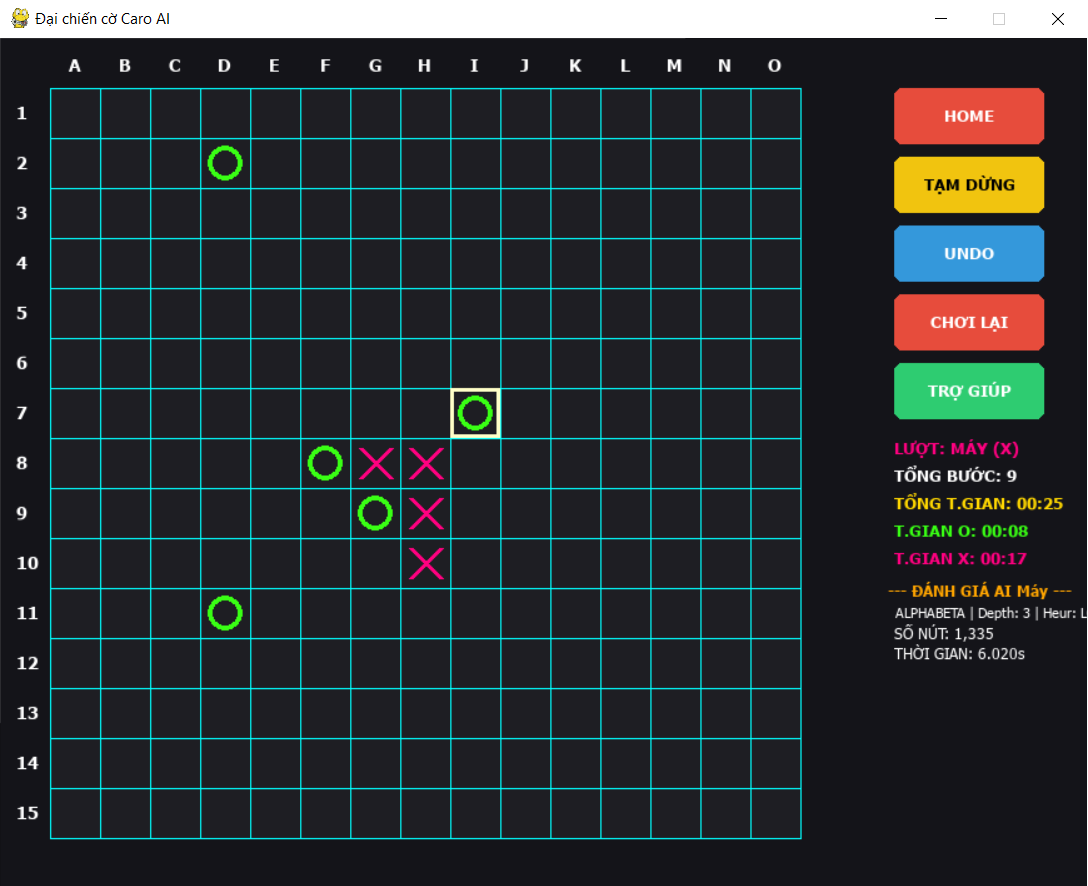
\includegraphics[width=\textwidth]{Figures/Gallery/play.png}
	\captionof{figure}{Giao diện trò chơi}
	\label{fig:gameplay}
\end{center}
\vspace{0.3cm}
\textbf{Đồ họa Neon:} Bàn cờ sử dụng lưới. Quân X (Hồng) và O (Xanh lá) nhằm tăng độ tương phản và chống mỏi mắt.

\textbf{Hệ thống Phản hồi trực quan:}
\begin{itemize}
	\item Tự động đánh dấu viền vàng cho nước đi mới nhất.
	\item Hiển thị viền cam nét đứt tại vị trí AI gợi ý đánh.
	\item Tạo hiệu ứng chớp nháy viền vàng làm nổi bật chuỗi 5 quân cờ chiến thắng.
\end{itemize}
\textbf{Xử lý trạng thái kết thúc:} Tự động ngắt nhạc nền, phát SFX Thắng/Thua. Quá trình giải phóng bộ nhớ và chuyển về Menu được kích hoạt mượt mà chỉ bằng một thao tác click chuột.
	
\begin{center}
	\nopagebreak
	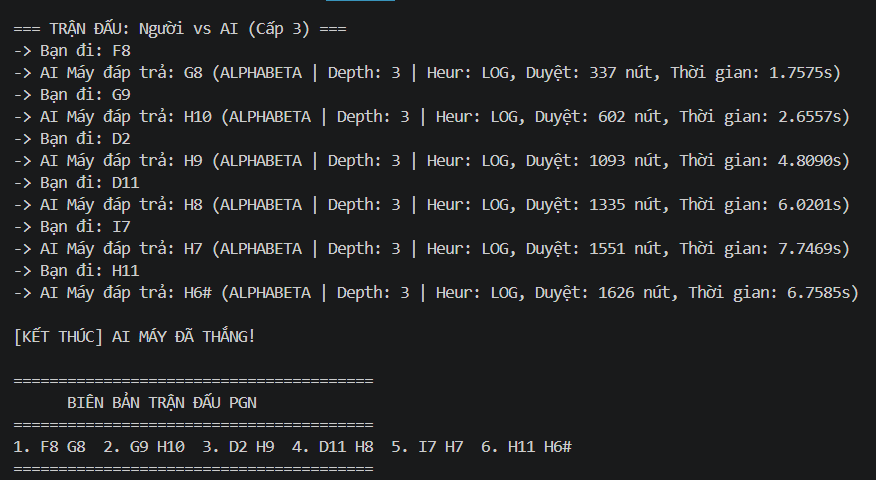
\includegraphics[width=\textwidth]{Figures/Gallery/result.png}
	\captionof{figure}{Màn hình Menu cấu hình chế độ chơi}
	\label{fig:result}
\end{center}
\vspace{0.3cm}
Hệ thống ghi nhận diễn biến trận đấu trên Terminal thông qua hai cơ chế:
\begin{itemize}
	\item In tọa độ từng nước đi theo thời gian thực (nước quyết định được đánh dấu).
	\item Xuất PGN: Tự động tổng hợp mảng lịch sử thành văn bản chuẩn PGN quốc tế ngay khi ván cờ kết thúc để phục vụ lưu trữ và phân tích.
\end{itemize}

\section{Các chỉ số đánh giá hiệu năng và năng lực của tác tử AI}

Để đánh giá một cách toàn diện hiệu quả của các kỹ thuật tối ưu hóa được đề xuất, nhóm thực hiện đề tài tiến hành nghiệm thu và khảo sát năng lực vận hành của hệ thống dựa trên cả hai phương diện: chỉ số hiệu năng tính toán định lượng và năng lực chiến thuật định tính.

\subsection{Khảo sát chỉ số hiệu năng tính toán thực tế (Định lượng)}
Nhóm chỉ số này đo lường mức độ tối ưu phần cứng và tốc độ xử lý của thuật toán tại các độ sâu tìm kiếm $d$ khác nhau thông qua môi trường đối kháng trực tiếp giữa Người và Máy (Human vs AI). 

Các tiêu chí định lượng bao gồm thời gian phản hồi trung bình cho một nước đi, tổng số nút trạng thái ma trận bàn cờ giả định mà CPU phải khởi tạo, duyệt thực tế và điểm số lượng giá tương ứng được chi tiết hóa tại Bảng \ref{tab:hieunang_thuc_te}.

\begin{table}[!htbp]
	\centering
	\renewcommand{\arraystretch}{1.3}
	\caption{Hiệu suất vận hành thực tế của giải thuật tích hợp theo từng cấp độ sâu}
	\label{tab:hieunang_thuc_te}
	\begin{tabular}{|c|c|c|l|}
		\hline
		\textbf{Cấp độ thiết lập} & \textbf{Thời gian phản hồi} & \textbf{Số nút duyệt thực tế} & \textbf{Năng lực tư duy (Định tính)} \\ \hline
		\textbf{Dễ ($d=1$)} & $\sim 0,008$ s & $5 \to 10$ nút & Sơ cấp\\ \hline
		\textbf{Vừa ($d=2$)} & $0,15 \to 0,8$ s & $100 \to 500$ nút & Trung bình\\ \hline
		\textbf{Khó ($d=3$)} & $0,15 \to 4,0$ s & $350 \to 3.500$ nút & Khá \\ \hline
		\textbf{Siêu khó ($d=4$)} & $\ge 3,0$ s & $\ge 2.500$ nút  & Cao cấp \\ \hline
	\end{tabular}
\end{table}

\paragraph{Nhận xét hệ số kiểm thử hiệu suất định lượng:}
\begin{itemize}
	\item \textbf{Sự bùng nổ tổ hợp trạng thái theo chiều sâu:} Đúng như quy luật toán học của cấu trúc cây quyết định, khi độ sâu tăng từ $d=1$ lên $d=4$, cả số lượng nút duyệt lẫn thời gian phản hồi đều tăng trưởng rõ rệt theo hàm mũ $\mathcal{O}(b^d)$ (với $b$ là hệ số nhánh cờ). Tại cấp độ Siêu khó ($d=4$), do không gian trạng thái giả lập quá lớn, thời gian tính toán có xu hướng kéo dài vượt ngưỡng $3,0$ giây ở giai đoạn trung cuộc. Điều này minh chứng cho tính đúng đắn của việc lựa chọn cấu hình mặc định $d=3$ ở giao diện hệ thống nhằm cân bằng tối ưu giữa năng lực tư duy thông minh và trải nghiệm thời gian thực của người dùng.
	\item \textbf{Hiệu quả của giải thuật thu hẹp vùng tìm kiếm:} Nhờ việc áp dụng hàm lọc nước đi tiềm năng \texttt{get\_interesting\_moves} để cô lập bán kính quét xung quanh các quân cờ hiện hành, số lượng nút duyệt ở cấp độ Khó ($d=3$) đã được kìm hãm thành công trong khoảng tuyến tính từ $350$ đến $3.500$ nút thay vì hàng triệu nút trên lý thuyết bàn cờ $15 \times 15$ vắng dòng lọc. Yếu tố này giúp thời gian phản hồi giữ vững ở mức tối ưu, hoàn toàn đáp ứng tiêu chuẩn mượt mà của một ứng dụng trò chơi tương tác.
\end{itemize}

\subsection{Khảo sát năng lực chiến thuật qua đối chiến giả lập (Định tính)}
Để đánh giá định tính năng lực xử lý chiến thuật và chứng minh sự tương quan trực tiếp giữa cấu hình thuật toán và kết quả thắng bại một cách tuyệt đối, hệ thống kích hoạt môi trường giả lập cho hai thực thể Bot tự đối đầu độc lập (AI vs AI) dưới hai kịch bản phân tách.

\textbf{Kịch bản 1: Khảo sát sự ảnh hưởng của chiều sâu cây quyết định ($d$)}

Thực nghiệm tiến hành cho hai tác tử sở hữu cùng thuật toán cải tiến hoàn chỉnh nhưng bất đối xứng về độ sâu tìm kiếm nhằm kiểm thử tính áp đảo hình học. Kết quả các cặp đấu đối kháng được thống kê tại Bảng \ref{tab:ai_vs_ai_depth}.

\begin{table}[!htbp]
	\centering
	\renewcommand{\arraystretch}{1.25}
	\caption{Ma trận kết quả đối đầu giữa các cấp độ sâu trên cùng giải thuật tích hợp}
	\label{tab:ai_vs_ai_depth}
	\begin{tabular}{|c|c|c|c|c|}
		\hline
		\textbf{Quân X $\backslash$ Quân O} & \textbf{$d = 1$} & \textbf{$d = 2$} & \textbf{$d = 3$} & \textbf{$d = 4$} \\ \hline
		\textbf{$d = 1$} & Quân O thắng & Quân O thắng & Quân O thắng & Quân O thắng \\ \hline
		\textbf{$d = 2$} & Quân X thắng & Quân O thắng & Quân O thắng & Quân O thắng \\ \hline
		\textbf{$d = 3$} & Quân X thắng & Quân X thắng & Quân O thắng & Quân O thắng \\ \hline
		\textbf{$d = 4$} & Quân X thắng & Quân X thắng & Quân X thắng & Quân O thắng \\ \hline
	\end{tabular}
\end{table}

\textbf{Kịch bản 2: Khảo sát năng lực xử lý giữa các tổ hợp biến thể giải thuật}

Thực nghiệm tiến hành cấu hình cố định độ sâu ở mức $d=2$ để tập trung kiểm thử tốc độ và khả năng dứt điểm trận đấu giữa các tầng kiến trúc logic cốt lõi bao gồm Minimax thuần túy, Minimax tích hợp Heuristic, và Minimax cải tiến hoàn chỉnh. Kết quả chi tiết tiến trình đối kháng được ghi nhận tại Bảng \ref{tab:ai_vs_ai_variants}.

\begin{table}[!htbp]
	\centering
	\renewcommand{\arraystretch}{1.25}
	\small
	\caption{Ma trận đối chiến và thời gian xử lý thực tế giữa các tổ hợp biến thể giải thuật ($d=2$)}
	\label{tab:ai_vs_ai_variants}
	\begin{tabular}{|m{3.5cm}|m{3.0cm}|m{3.3cm}|m{4.2cm}|}
		\hline
		\textbf{Quân X $\backslash$ Quân O} & \textbf{Minimax thuần túy} & \textbf{Minimax + Heuristic} & \textbf{Minimax + Alpha-Beta + Heuristic} \\ \hline
		\textbf{Minimax thuần túy} & X thắng \newline ($t: 0.001\text{s} \to 0.5\text{s}$ cả X, O) & O thắng \newline ($t: 0.001\text{s} \to 0.5\text{s}$ quân X \newline $0.09\text{s} \to 0.64\text{s}$ quân O) & O thắng \newline ($t: 0.001\text{s} \to 0.5\text{s}$ quân X \newline $0.01\text{s} \to 0.56\text{s}$ quân O) \\ \hline
		\textbf{Minimax + Heuristic} & X thắng \newline ($t: 0.001\text{s} \to 0.5\text{s}$ quân O \newline $0.13\text{s} \to 0.77\text{s}$ quân O) & O thắng \newline ($t: 1\text{s} \to 7\text{s}$ cả X, O) & O thắng \newline ($t: 0.14\text{s} \to 2.8\text{s}$ quân X \newline $0.15\text{s} \to 0.4\text{s}$ quân O) \\ \hline
		\textbf{Minimax + Alpha-Beta + Heuristic} & X thắng \newline ($t: 0.001\text{s} \to 0.5\text{s}$ quân X \newline $0.06\text{s} \to 0.52\text{s}$ quân O) & O thắng \newline ($t: 1\text{s} \to 7\text{s}$ quân O \newline $0.15\text{s} \to 0.4\text{s}$ quân X) & O thắng \newline ($t: 0.15\text{s} \to 1.8\text{s}$ cả X, O) \\ \hline
	\end{tabular}
\end{table}

\paragraph{Nhận xét chuyên sâu từ kết quả đối chiến giả lập:}
\begin{itemize}
	\item \textbf{Sự áp đảo của chiều sâu duyệt cây (Depth):} Minh chứng từ Bảng \ref{tab:ai_vs_ai_depth} chỉ ra rằng khi có sự chênh lệch về độ sâu tìm kiếm, tác tử sở hữu cấu hình độ sâu cao hơn luôn giành chiến thắng tuyệt đối trước tác tử có độ sâu thấp hơn. Khả năng nhìn xa giúp Bot phát hiện và bẻ gãy các chuỗi triển khai cờ tiềm năng của đối thủ ngay từ giai đoạn sơ khởi.
	\item \textbf{Lợi thế đi trước (First-player Advantage):} Một đặc trưng hình học quan trọng của cờ Caro được mô hình hóa rõ nét thông qua thực nghiệm: Khi hai tác tử đồng cấp về cả thuật toán lẫn độ sâu đối đầu trực diện, phần thắng luôn thuộc về thực thể được cấu hình cầm quân O (đi trước). Áp lực chủ động tấn công liên tục từ nước đi đầu tiên giúp phe tiên phong tối ưu hóa tỷ lệ dứt điểm ván đấu.
	\item \textbf{Tính tất định của hệ thống (Deterministic):} Các ván đấu giả lập EvE cho thấy nếu giữ nguyên cấu hình tham số đầu vào, diễn biến trận đấu sẽ lặp lại chính xác $100\%$ y hệt nhau giữa các lần chạy. Hệ thống hoàn toàn không bị nhiễu bởi các yếu tố ngẫu nhiên, khẳng định tính ổn định vững chắc của hàm lượng giá tĩnh Heuristic.
	\item \textbf{Sự cải thiện vượt bậc về hiệu năng nhờ Alpha-Beta:} Dựa trên Bảng \ref{tab:ai_vs_ai_variants}, việc tích hợp thêm kỹ thuật cắt tỉa Alpha-Beta vào lõi lọc Heuristic đã chứng minh hiệu quả giảm tải tài nguyên thần kỳ. Thời gian phản hồi của nước đi được rút ngắn từ ngưỡng nguy hiểm ($1\text{s} \to 7\text{s}$) xuống mức lý tưởng ($0.15\text{s} \to 0.4\text{s}$), làm phẳng đồ thị trồi sụt toán học và giải quyết triệt để bài toán thắt nút cổ chai xử lý của CPU.
\end{itemize}

% =================================================================
%   MỤC 4.3: HẠN CHẾ CỦA HỆ THỐNG
% =================================================================
\section{Hạn chế của hệ thống hiện tại}

Mặc dù hệ thống đã đạt được những kết quả khả quan về mặt tốc độ phản hồi và có thể đánh bại người chơi ở mức độ trung bình, tác tử AI vẫn tồn tại một số hạn chế kỹ thuật cốt lõi do đặc thù của giải thuật Heuristic tĩnh:

\begin{itemize}
	\item \textbf{Chưa nhận diện được các đòn chiến thuật nước đôi, nước ba phức tạp:} Do hàm Heuristic hoạt động theo cơ chế quét mẫu hình tĩnh (\textit{static pattern matching}) độc lập cho từng hướng, Bot chỉ nhận biết được độ nguy hiểm khi các quân cờ đã đứng cạnh nhau tạo thành chuỗi. Khi đối thủ sử dụng các đòn chiến thuật nâng cao như \textbf{nước đôi} (tạo ra hai hàng 3 hoặc hai hàng 4 đồng thời ở hai hướng khác nhau từ một nước đi) hoặc \textbf{đòn phân nhánh mở rộng}, Bot thường bị động và không thể nhận diện được hiểm họa từ các nước đi chuẩn bị từ xa.
	
	\item \textbf{Hiện tượng mù chân trời (\textit{Horizon Effect}):} Do giới hạn năng lực phần cứng, độ sâu duyệt tối ưu trong thời gian thực chỉ đạt tới $d = 4$ hoặc $d = 5$. Nếu đối thủ thiết lập một bẫy cờ kết thúc ván đấu ở nước thứ $6$ hoặc $7$ (nằm ngoài tầm nhìn của độ sâu $d$), Bot hoàn toàn "mù" trước hiểm họa này và sẽ đưa ra các nước đi thiển cận ở lượt hiện tại.
	
	\item \textbf{Sự trùng lặp tính toán do thiếu cấu trúc dữ liệu lưu vết nâng cao:} Hệ thống hiện tại chưa triển khai cấu trúc dữ liệu Bảng chuyển vị (\textit{Transposition Table}). Trong cờ Caro, việc hạ các quân cờ ở các thứ tự đảo mảng khác nhau hoàn toàn có thể dẫn đến một trạng thái cấu trúc ma trận bàn cờ trùng lặp tuyệt đối. Do thiếu bộ nhớ đệm (\textit{Cache}), Bot vẫn phải thực thi tính toán đệ quy lại từ đầu cho các nhánh tương đương này, gây lãng phí một lượng tài nguyên xử lý cực kỳ lớn của CPU.
	
	\item \textbf{Sự phụ thuộc vào quy mô dữ liệu huấn luyện của ma trận điểm Machine Learning:} Mặc dù phương pháp tối ưu hóa bằng Hồi quy Logistic bước đầu đã tự động hóa việc trích xuất điểm số thực nghiệm có độ mịn cao, bộ trọng số vẫn bị giới hạn bởi quy mô của tập dữ liệu mẫu ban đầu. Trong một số biến thể cờ thế phức tạp chưa xuất hiện trong tập huấn luyện, tác tử AI sử dụng cấu hình điểm này vẫn có xác suất đưa ra các quyết định chưa đạt mức tối ưu tuyệt đối.
\end{itemize}